\chapter{Modelli di produzione software}

\section{Modelli a cascata}

\paragraph{Modello waterfall} Susseguirsi sequenziale di fasi aventi come output un \textit{deliverable} (input per la fase successiva). Processo disciplinato, documentato, ben pianificato e gestibile. L'implementazione è rimandata alla definizione chiara degli obiettivi. Risulta \textit{rigido e monolitico}, non presenta \textit{feedback e parallelismo} e prevede un unica data di consegna.

\begin{figure}[h!]
  \centering
  \subfloat[Classico]{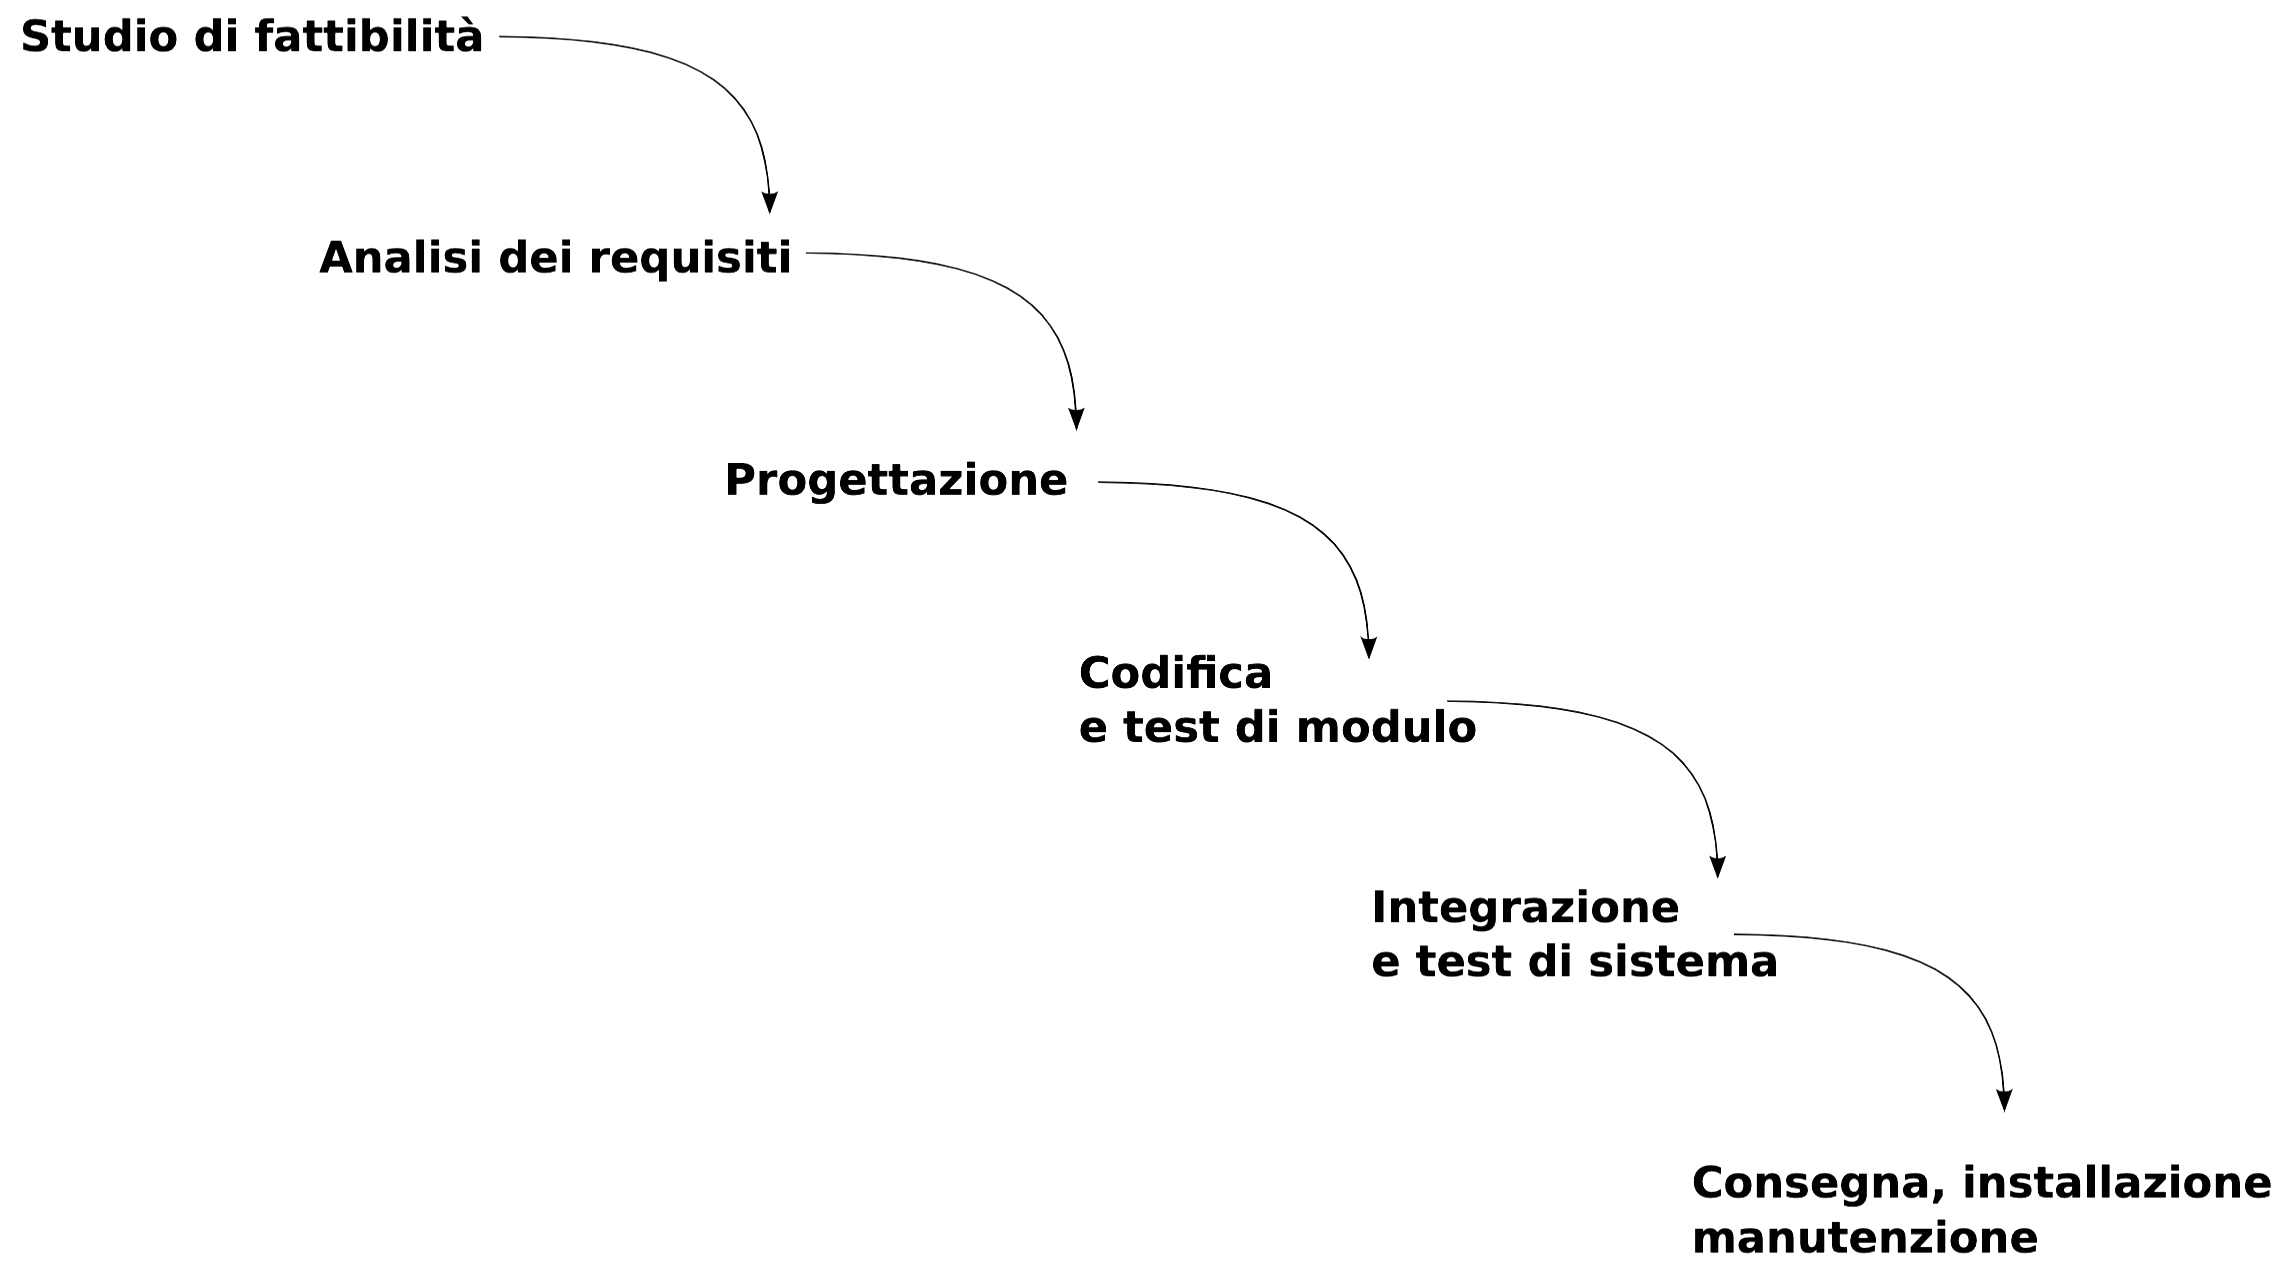
\includegraphics[width=0.48\textwidth]{assets/waterfall.png}}\label{fig:waterfall}
  \hfill
  \subfloat[Con feedback]{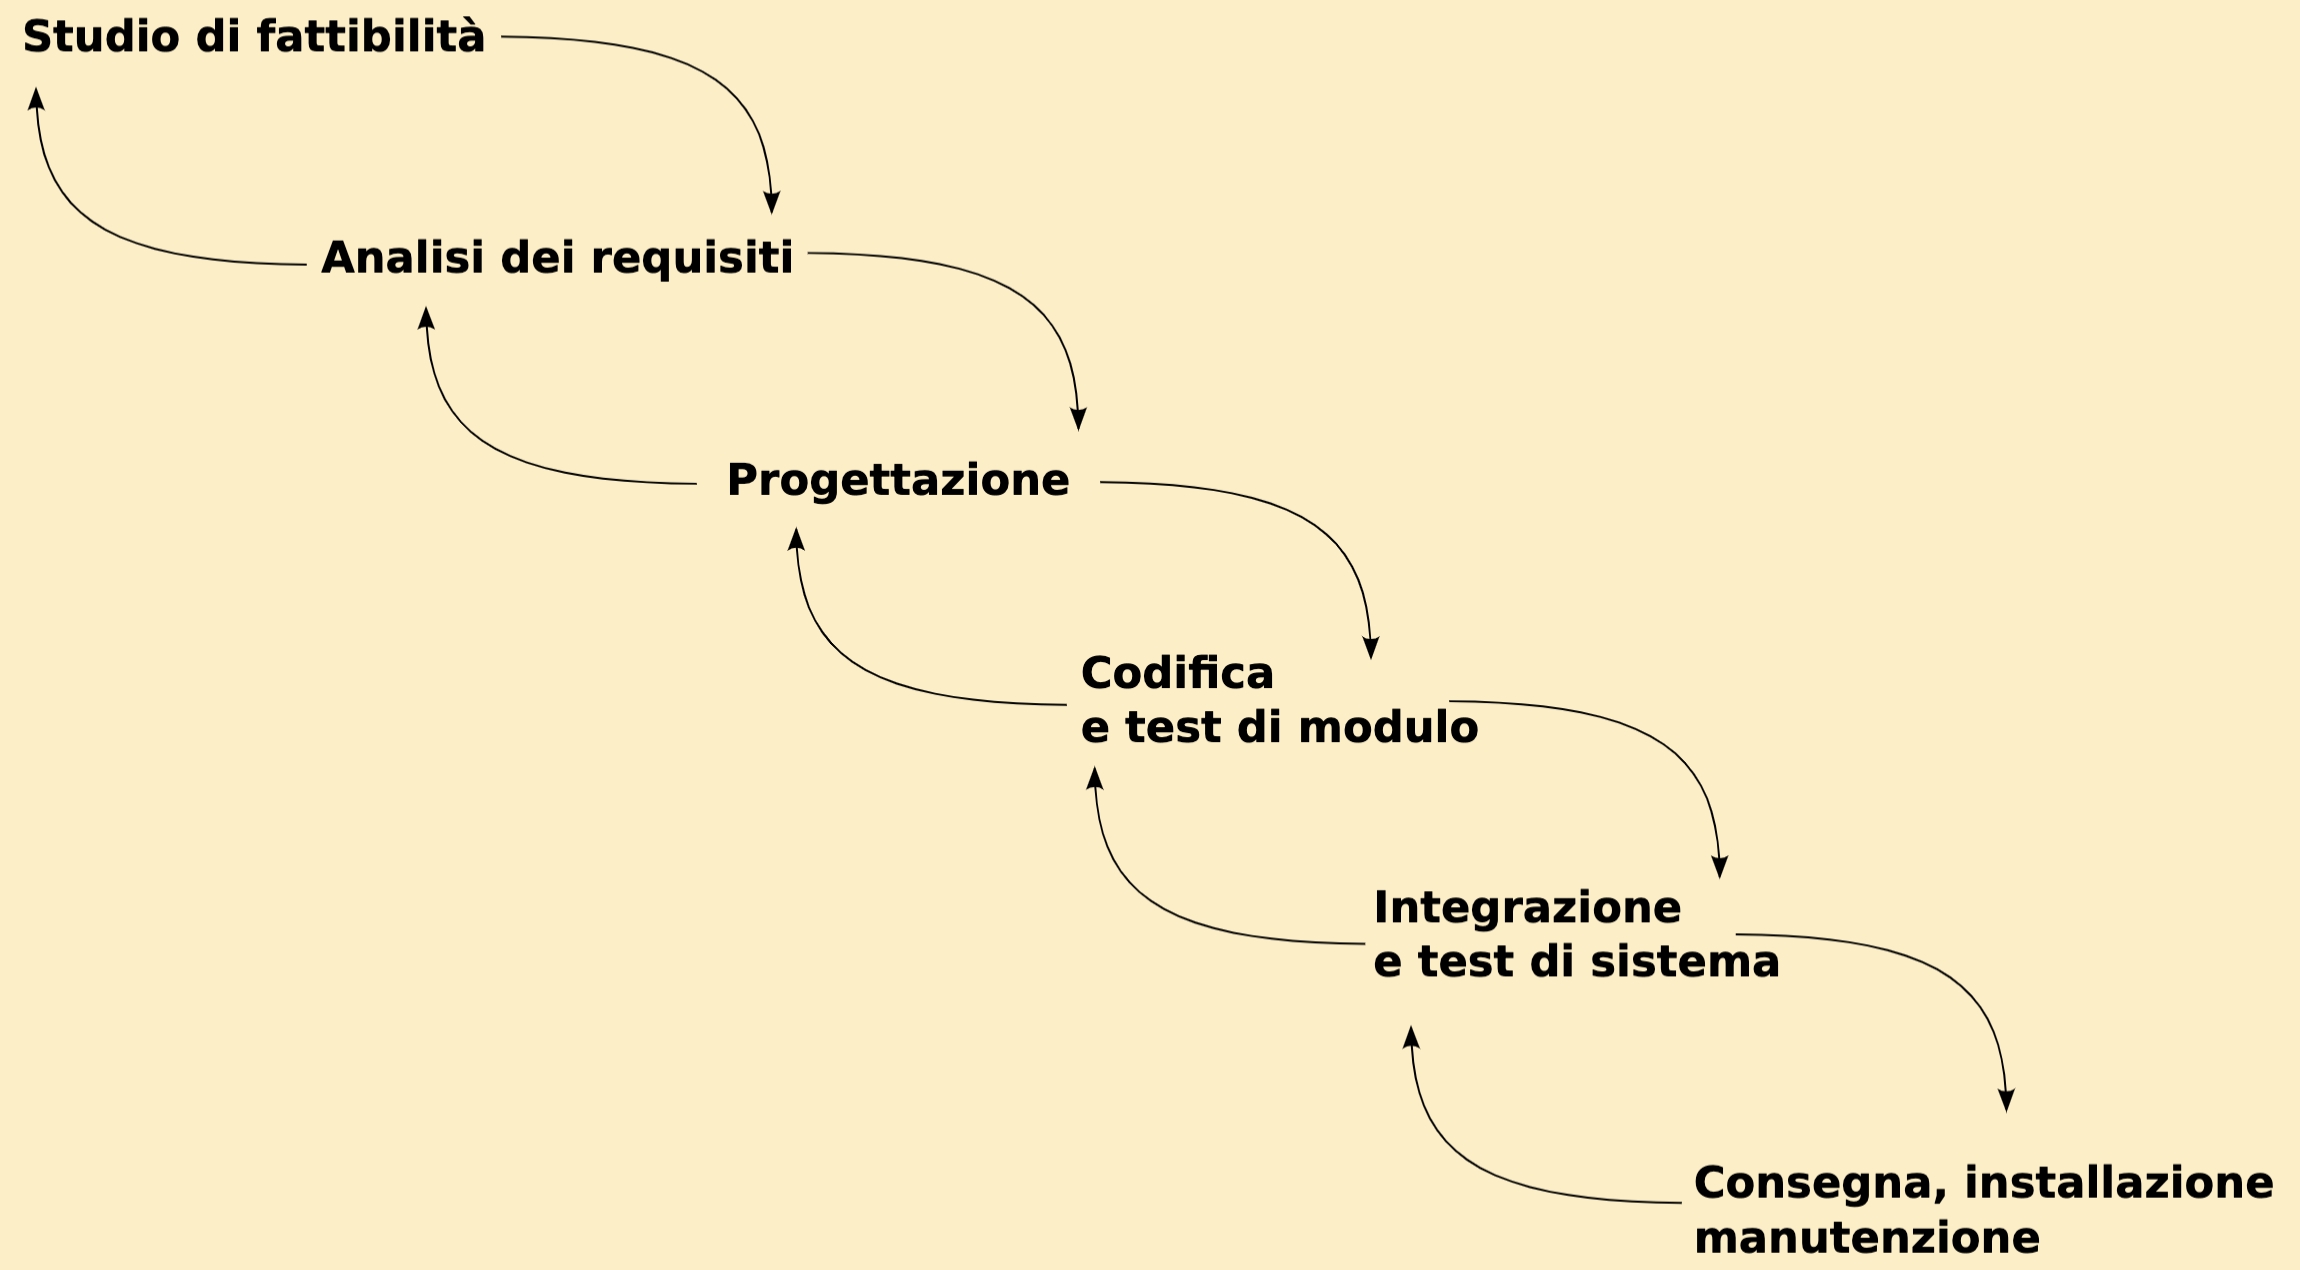
\includegraphics[width=0.48\textwidth]{assets/waterfall_fb.png}}\label{fig:waterfall-fb}
  \caption{Modelli a cascata}
\end{figure}

\paragraph{Modello con feedback} Risolve il problema dell'assenza di feedback, limitandolo tra una fase e quella successiva. Presenta limitazioni:
\begin{itemize}
    \item Non è possibile tener conto di nuove informazioni evidenziate (uscite fuori) in fasi di sviluppo avanzate;
    \item È difficile identificare TUTTI i requisiti una sola volta (è sbagliato assumere che non cambino nel tempo).
\end{itemize}


\newpage

\section{Modelli incrementali}

In generale i modelli a cascata non si prestano all'anticipazione del cambiamento, motivo per cui \textbf{\textit{Boehm}} teorizzò il \textit{modello evolutivo} (o \textit{incrementale}) in cui le fasi consistono in \textit{versioni incrementali} di un prodotto software operazionale, con una direzione evolutiva determinata dall'esperienza pratica. Si ottiene quindi una prima versione funzionante (prototipo cestinabile o \textit{throw-away}, secondo il principio "do it twice") sottoposta alla valutazione degli stakeholder, per poi sviluppare una nuova versione rilasciabile che raccoglie i feedback dei clienti. La \textit{strategia evolutiva} consiste in:
\begin{enumerate}
    \item \textbf{Rilascio} di una funzionalità all'utente
    \item \textbf{Misura} del valore aggiunto per il cliente
    \item \textbf{Aggiustamento} del progetto e degli obiettivi
\end{enumerate}

\begin{figure}[h!]
    \centering
    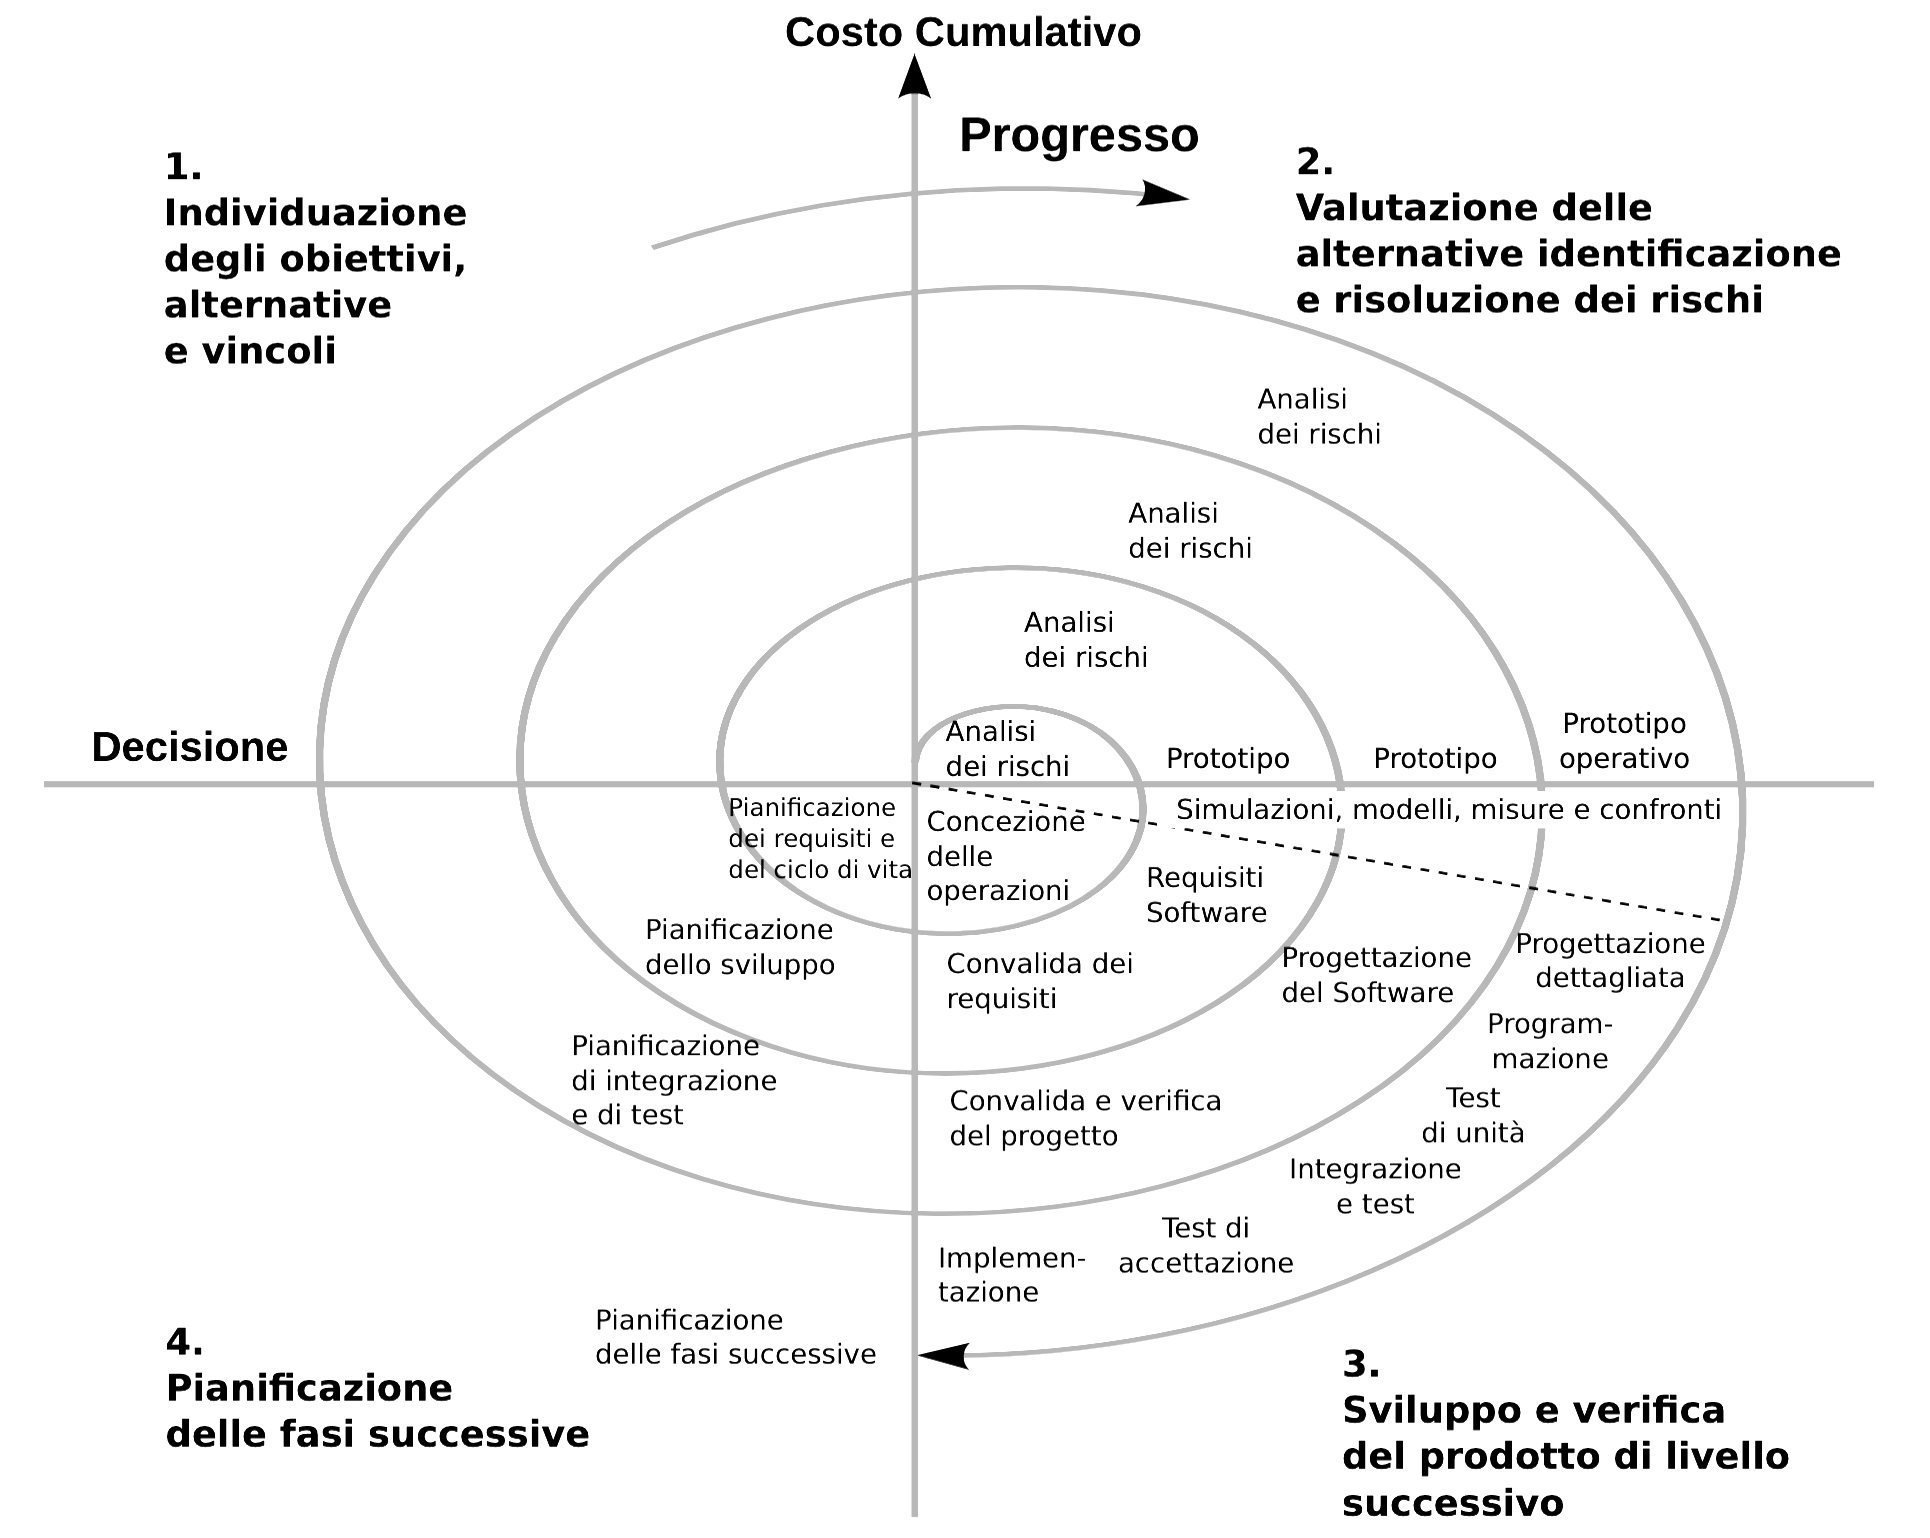
\includegraphics[width=0.75\linewidth]{assets/spirale.png}
    \caption{Modello a spirale}
    \label{fig:modello-spirale}
\end{figure}

\paragraph{Modello a spirale} Composto di quattro fasi cicliche:
\begin{enumerate}
    \item Individuazione di obiettivi, strategie e vincoli
    \item Valutazione dei rischi e delle alternative
    \item Sviluppo e verifica
    \item Revisione e pianificazione (per la prossima fase)
\end{enumerate}
Il \textbf{raggio} della spirale corrisponde al \textit{costo accumulato}, l'\textbf{angolo} rappresenta il \textit{progresso}

\section{Casi Studio}

\paragraph{Microsoft - Synchronize and Stabilize} Si scompone il progetto complesso in piccole squadre che lavorano in parallelo, affrontando tutte le fasi dello sviluppo. Si inizia con una \textit{fase di pianificazione} avente come output un documento di specifica (aggiornabile). Si procede a \textit{rilasci incrementali}. Alla fine di ogni giornata si ha la fase di \textbf{sincronizzazione}: ogni team inserisce i risultati del lavoro svolto in un database, si integrano i componenti sviluppati (\textit{build}) e si compila e testa il codice. L'ultima fase prevede la definizione di date (\textit{milestone}) di \textbf{stabilizzazione}: congelamento momentaneo delle specifiche (\textit{feature freeze}) per risolvere errori e consolidare il codice sviluppato. 

\paragraph{Software Open-Source} Rilasciati sotto \textit{licenze copyleft} (es. GPL) che non pongono restrizioni sull'acquisizione, lo studio, la modifica o la redistribuzione del codice, a patto che ogni eventuale rilascio avvenga sotto lo stesso regime giuridico. La tecnica si basa su \textbf{collaborazione} tra programmatori, \textbf{comunicazione} (tramite e-mail o gruppi di discussione) e \textbf{condivisione} del codice (tramite VCS). Si hanno pochi sviluppatori (o maintainers, lungo termine) e tanti contributori (breve termine, posso diventare sviluppatori)

\section{Unified Software Development Process}
Seguire una metodologia presenta alcuni vantaggi (come la riduzione dei tempi di sviluppo, il miglioramento della comunicazione nel team, ecc...), ma la maggior parte di esse non ha una solida base teoria, ma è supportata empiricamente dal buon senso. Non è  possibile seguirla in ogni situazione.

\paragraph{Unified Software Development Process (UP)} Metodologia basata sul paradigma POO e sul linguaggio di modellazione UML. UP prevede una ripetizione di \textit{cicli di sviluppo controllati}, ciascuno dei quali termina con il rilascio di una versione incrementale (prototipo intermedio) del prodotto.

\begin{figure}[h!]
    \centering
    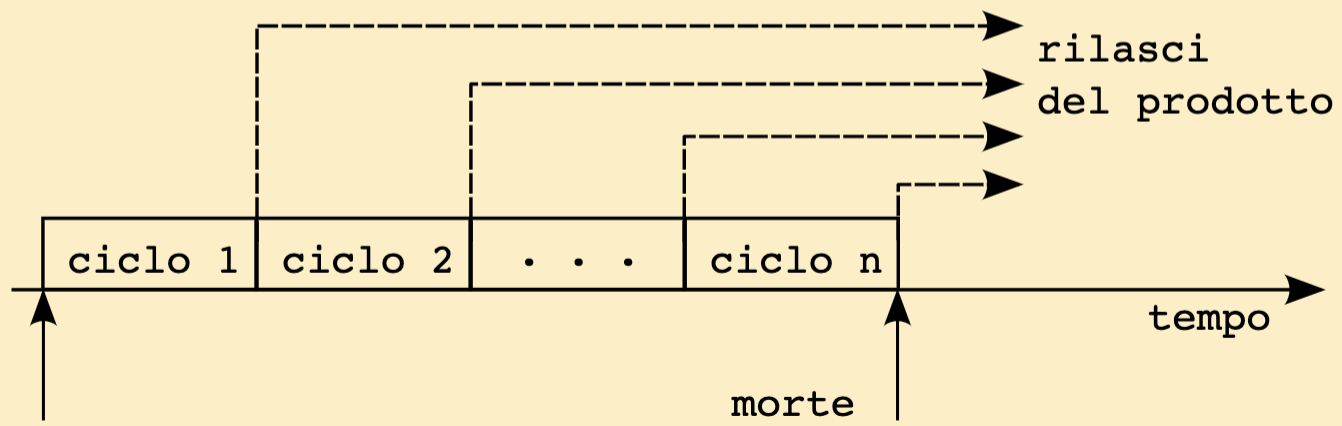
\includegraphics[width=0.75\linewidth]{assets/up.png}
    \caption{Cicli di sviluppo}
    \label{fig:cicli-up}
\end{figure}

\newpage

\paragraph{Rational Unified Process (RUP)} Ogni ciclo è diviso in quattro fasi (ognuna delle quali termina con una \textit{milestone}, un insieme di artefatti suscettibili a controllo qualità):
\begin{enumerate}
    \item \textbf{Concezione}: valutazione della fattibilità del progetto;
    \item \textbf{Elaborazione}: specifica degli use-case e dell'architettura software (\textit{baseline})
    \item \textbf{Costruzione}: implementazione del codice e testing di funzionalità
    \item \textbf{Transizione}: rilascio prototipale (disribuzione, formazione utenti, beta testing, ecc...)
\end{enumerate}

\begin{figure}[h!]
    \centering
    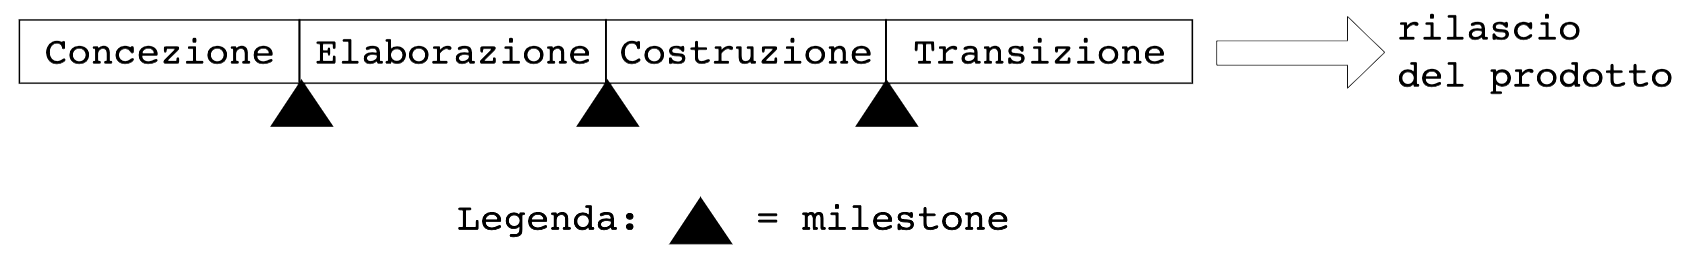
\includegraphics[width=0.75\linewidth]{assets/rup.png}
    \caption{Fasi dei cicli di sviluppo}
    \label{fig:fasi-rup}
\end{figure}

Ogni fase è suddivisa in una serie di iterazioni (ognuna delle quali produce un incremento valutabile). Le attività del processo di sviluppo (o \textit{workflow)} sono svolte parallelamente in ogni iterazione. Questa metodologia è guidata dai \textit{casi d'uso} e centrata sulle \textit{architetture}. Incoraggia uno sviluppo incrementale basato sulle priorità del cliente e sull'utilizzo di componenti riusabili (\textit{architetture component-based}).

\begin{figure}[h!]
    \centering
    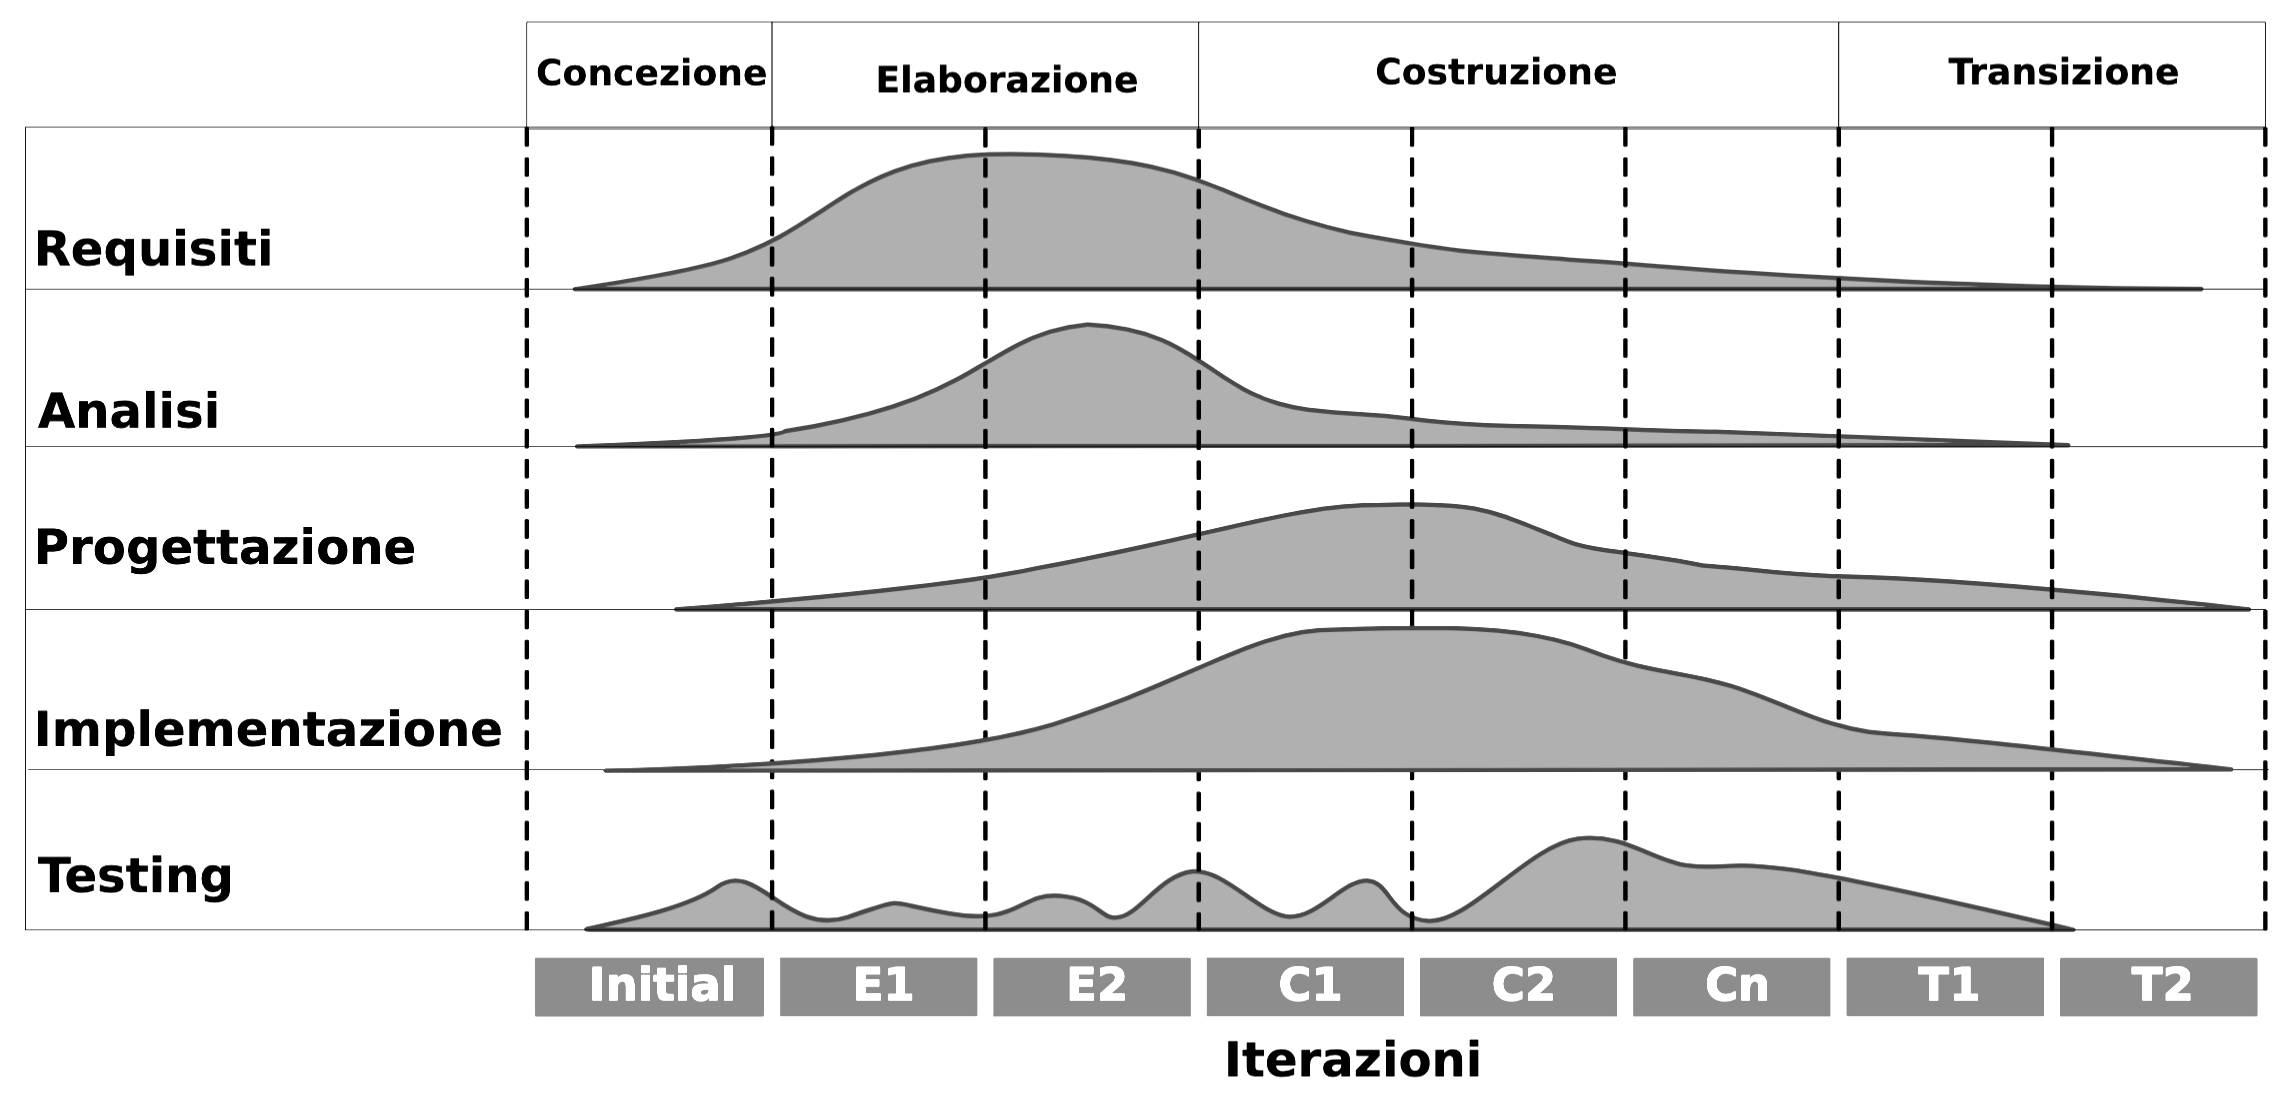
\includegraphics[width=0.75\linewidth]{assets/rup_workflow.png}
    \caption{Workflow con fasi ed iterazioni}
    \label{fig:rup-workflow}
\end{figure}

\newpage

\section{Metodologie agili, Extreme programming e Scrum}

Le metodologie di sviluppo tradizionali (\textit{plan-based}) prevedono: pianificazione iniziale (requisiti), individuazione delle fasi di produzione e definizione anticipata dell'output di ciascuna fase. Non sono adatte agli ambienti moderni in cui i requisiti sono in \textit{continua e rapida evoluzione}.

\begin{figure}[h!]
    \centering
    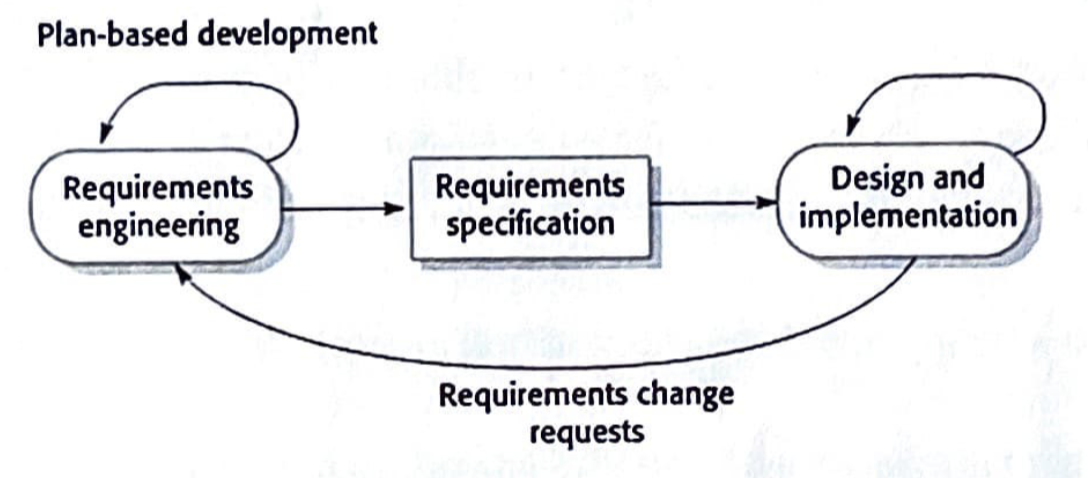
\includegraphics[width=0.75\linewidth]{assets/plan-based.png}
    \caption{Sviluppo plan-based}
    \label{fig:plan-based-dev}
\end{figure}

Il focus si sposta quindi su: rapidità di sviluppo e rilascio del prodotto software; capacità di rispondere ai cambiamenti dei requisiti senza \textit{overhead} (eccessivo carico di lavoro). Nascono per questi motivi le \textit{\textbf{metodologie di sviluppo agili}}, caratterizzate dall\textit{interfogliamento} delle attività di specifica, progettazione, implementazione e testing. Si elimina il bisogno di pianificazione e documentazione statica dei requisiti.

\begin{figure}[h!]
    \centering
    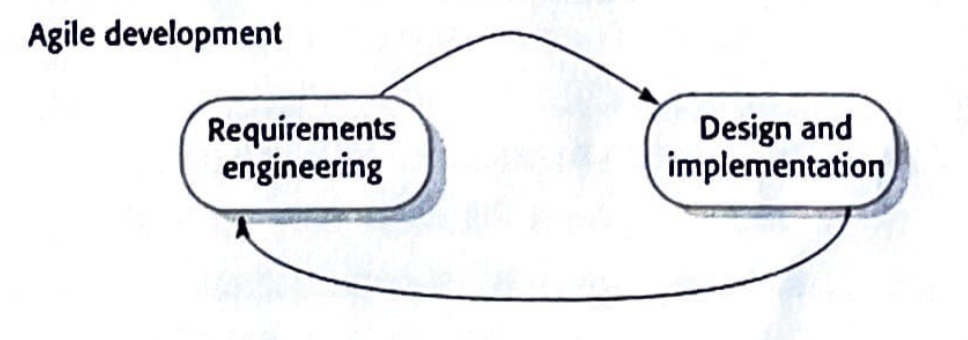
\includegraphics[width=0.75\linewidth]{assets/agile-dev.png}
    \caption{Sviluppo agile}
    \label{fig:agile-dev}
\end{figure}

\newpage

Secondo l'\textbf{\textit{Agile Manifesto}} (2001): “\textit{We are uncovering better ways of developing software by doing it and helping other to do it. Through this work we hove come to value:
\begin{itemize}
    \item Individual and interactions over processes and tools;
    \item Working software over comprehensive documentation;
    \item Customer callaboration over contract negotiation;
    \item Responding to change over following a plan;
\end{itemize}
That is, while there is value in the items on the right, we value the items on the left more}”


I \textbf{principi} alla base dei metodi agili sono:
\begin{enumerate}

    \item \textbf{Evoluzione} incrementale del sistema (sviluppo e rilascio iterativo)
    \item Intenso \textbf{coinvolgimento degli stakeholder} (nella definizione dei requisiti e valutazione di ogni iterazione)
    \item Focalizzazione sul \textbf{codice} (meno progettazione e documentazione)
    \item Valorizzazione delle \textbf{risorse umane} (il team non viene obbligato a seguire procedure standard)
    \item \textbf{Progettazione evolutiva} del sistema (“\textit{Embrace the change!}”)
    \item \textbf{Semplicità} nel codice e nella struttura del sistema.
\end{enumerate}
Si fa intensivo uso di \textbf{tool automatizzati} (es. testing). Sono ideali per lo sviluppo di prodotti di \textit{piccole/medie dimensioni}, dove è possibile coinvolgere il committente e il processo di produzione non è soggetto a rigide leggi o regolamentazioni esterne.


\paragraph{Extreme Programming (XP)} Una delle più importanti tecniche agili, porta il concetto di \textit{sviluppo incrementale} all'estremo, si possono produrre più versioni anche nello stesso giorno; ogni due settimane si rilascia ai clienti (se il testing ha successo). Si segue il seguente ciclo:
\begin{enumerate}
    \item Individuazione delle \textit{storie dell'utente} (scenari di utilizzo)
    \item Scomposizione delle storie in \textit{task} (operazioni che il sistema deve eseguire)
    \item Pianificazione dello sviluppo; suddivisione del lavoro
    \item Implementazione, integrazione e testing del sistema
    \item Rilascio della nuova \textit{build} ai clienti
    \item Valutazione della versione rilasciata
\end{enumerate} Le pratiche più importanti dell'XP sono:
\begin{itemize}
    \item \textbf{User stories for specification}: scenari di utilizzo raccolti in \textit{storie scritte}, classificate in base alla priorità per il committente e accompagnate da una stima di costi e carico di lavoro per l'implementazione dei task associati. Favorisce la \textit{pianificazione incrementale}, si da priorità alle funzionalità essenziali proseguendo con rilasci (non corposi, ma rapidi) di versioni che implementano nuove funzionalità o ne migliorano altre.
    \item \textbf{Refactoring}: revisione continua del software per introdurre miglioramenti, mantenendo una progettazione semplice e comprensibile. Favorisce \textit{anticipazione del cambiamento}, manutenibilità ed evolvibilità.
    \item \textbf{Test-first development}: si effettuano continui \textbf{test di specifica} tramite framework o tool automatici (es. \textit{Junit}) per ogni funzionalità prima di implementarla. Si procede con tecniche di \textit{testing incrementale}: i nuovi componenti sono simulati tramite componenti \textit{stand-alone}, le componenti preesistenti tramite \textit{test di regressione}. Completezza e correttezza sono difficili da garantire, si raggruppano gli input in gruppi che portano il sistema a comportarsi in maniera simile. Si testano anche i casi \textit{ai bordi}.
    \item \textbf{Pair programming}: si sviluppa il codice in coppie (di sviluppatori, cambiano dinamicamente favorendo collaborazione e condivisione delle conoscenze) che integrano più parti (a scelta) del sistema. È compito dell'uno controllare l'altro.
    \item \textbf{Customer involvement}: si sceglie un utente (tra gli utilizzatori finali) che faccia da rappresentante nel team, disponibile a: fornire requisiti, decidere la loro progettazione, contribuire alla definizione dei test e alla validazione dei risultati.
\end{itemize}
Tutto sommato, l'XP è una tecnica difficile da applicare, motivo per cui spesso si tende ad applicare solo singole pratiche a scapito dell'intera tecnica.

\paragraph{Guida Scrum} È una metodologia di gestione (\textit{project management}) agile ottimizzata per lo sviluppo incrementale (adatta a team con non più di 7 sviluppatori con unica sede). È costituita da tre fasi:
\begin{enumerate}
    \item \textbf{Pianificazione iniziale} in cui si stabiliscono obiettivi generali e architettura del sistema. Requisiti, specifiche, scenari d'utilizzo e task vengono raccolti nel \textbf{\textit{product backlog}} (una sorta di \textit{todo-list}), costantemente revisionato ed aggiornato dal \textit{product owner} (persona o gruppo che rappresenta gli stakeholder, non indicato dalla guida, generico per metodologie agili), il quale individua esigenze di mercato e priorità tra le specifiche;
    \item \textbf{Sprint cycle}: serie di iterazioni di sviluppo (con durata fissa 2/4 settimane), ciascuna delle quali produce un incremento \textit{potentially shippable} (pronto ad essere integrato). Durante i cicli il team si riunisce (incontri detti "scrum") in cui si revisiona il lavoro, si scambiano informazioni, si discute di eventuali problemi e si pianificano le prossime iterazioni. Con il termine \textit{velocity} si indica la stima della porzione di product backlog che il team è in grado di completare in un singolo sprint: se sovrastimata il team sarà sottoposto ad  \textit{overhead}, se sottostimata il ritmo di produzione non sarà efficiente, se ben calcolata il progetto viene scomposto in porzioni gestibili dal team;
    \item \textbf{Fase conclusiva} in cui: si apportano le ultime modifiche (dettagli) al prodotto in vista del rilascio finale e si scrive la documentazione necessaria (es. manuale utente).
\end{enumerate}

\begin{figure}[h!]
    \centering
    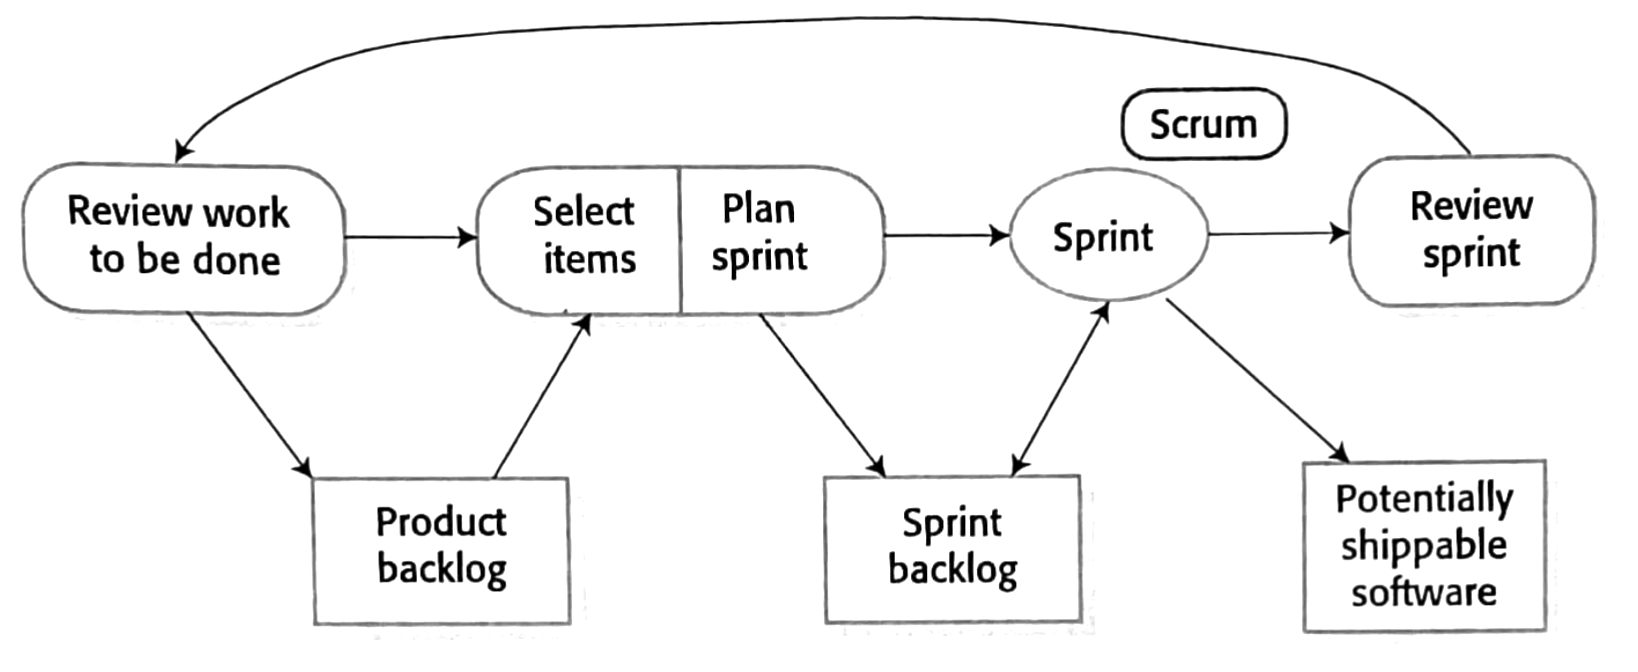
\includegraphics[width=0.75\linewidth]{assets/sprint-cycle.png}
    \caption{Ciclo Scrum}
    \label{fig:sprint-cycle}
\end{figure}

Durante uno sprint le comunicazioni da e verso l'esterno sono mediate dallo \textbf{\textit{scrum master}}: individuo che guida il lavoro del gruppo e si assicura che esso segua i principi di Scrum. Può essere visto come un \textit{facilitatore} al servizio del team.

\paragraph{Distributed Scrum} Permette un team sparso in diverse locazioni: si concorda una piattaforma di sviluppo comune la comunicazione avviene tramite messaggi, e-mail e videochiamate.

\paragraph{Multi-team Scrum} Coinvolge più team indipendenti aventi propri \textit{product owner} e \textit{scrum master}. Ogni team sviluppa una porzione distinta del software. I \textbf{\textit{product architects}} si occupano dell'architettura complessiva del sistema. Giornalmente i rappresentanti di ogni team si riuniscono per una pianificazione collettiva (“\textit{scrum of scrum}”)

\subsection{Scalabilita delle metodologie agili}

\paragraph{Scaling Up} È possibile applicare i metodi e le tecniche agili alla produzione di sistemi software di grandi dimensioni e con lunghi tempi di progetto?

\paragraph{Scaling Out} È possibile introdurre metodi e tecniche agili in aziende di grosse dimensioni e con alle spalle una diversa tradizione di sviluppo software?

\paragraph{Criticità} Le metodologie agili presentano le seguenti criticità:
\begin{enumerate}
    \item L'\textbf{informalità} le rende poco compatibili con approcci legali (comuni in grandi aziende che hanno ad esempio enti pubblici come committenti).
    \item La \textbf{contrattualizzazione} del software non è adatta all'evolvibilità delle metodologie agili, ma solo ai tempi di sviluppo (questione rischiosa per grandi committenti)
    \item La \textbf{scarsa documentazione} e il forte \textbf{anticipamento del cambiamento} non sono adatti ad un mantenimento a lungo termine
    \item I \textbf{rilasci incrementali} presentano criticità evidenti in prodotti software di grandi dimensioni
    \item Poca flessibilità nei confronti di \textbf{software preesistenti} (“\textit{brownfield systems}”)
    \item La \textbf{coordinazione tra team} risulta difficoltosa poiché i grandi sistemi sono spesso sviluppati come \textbf{progetti separati}.
\end{enumerate}

\begin{figure}[h!]
    \centering
    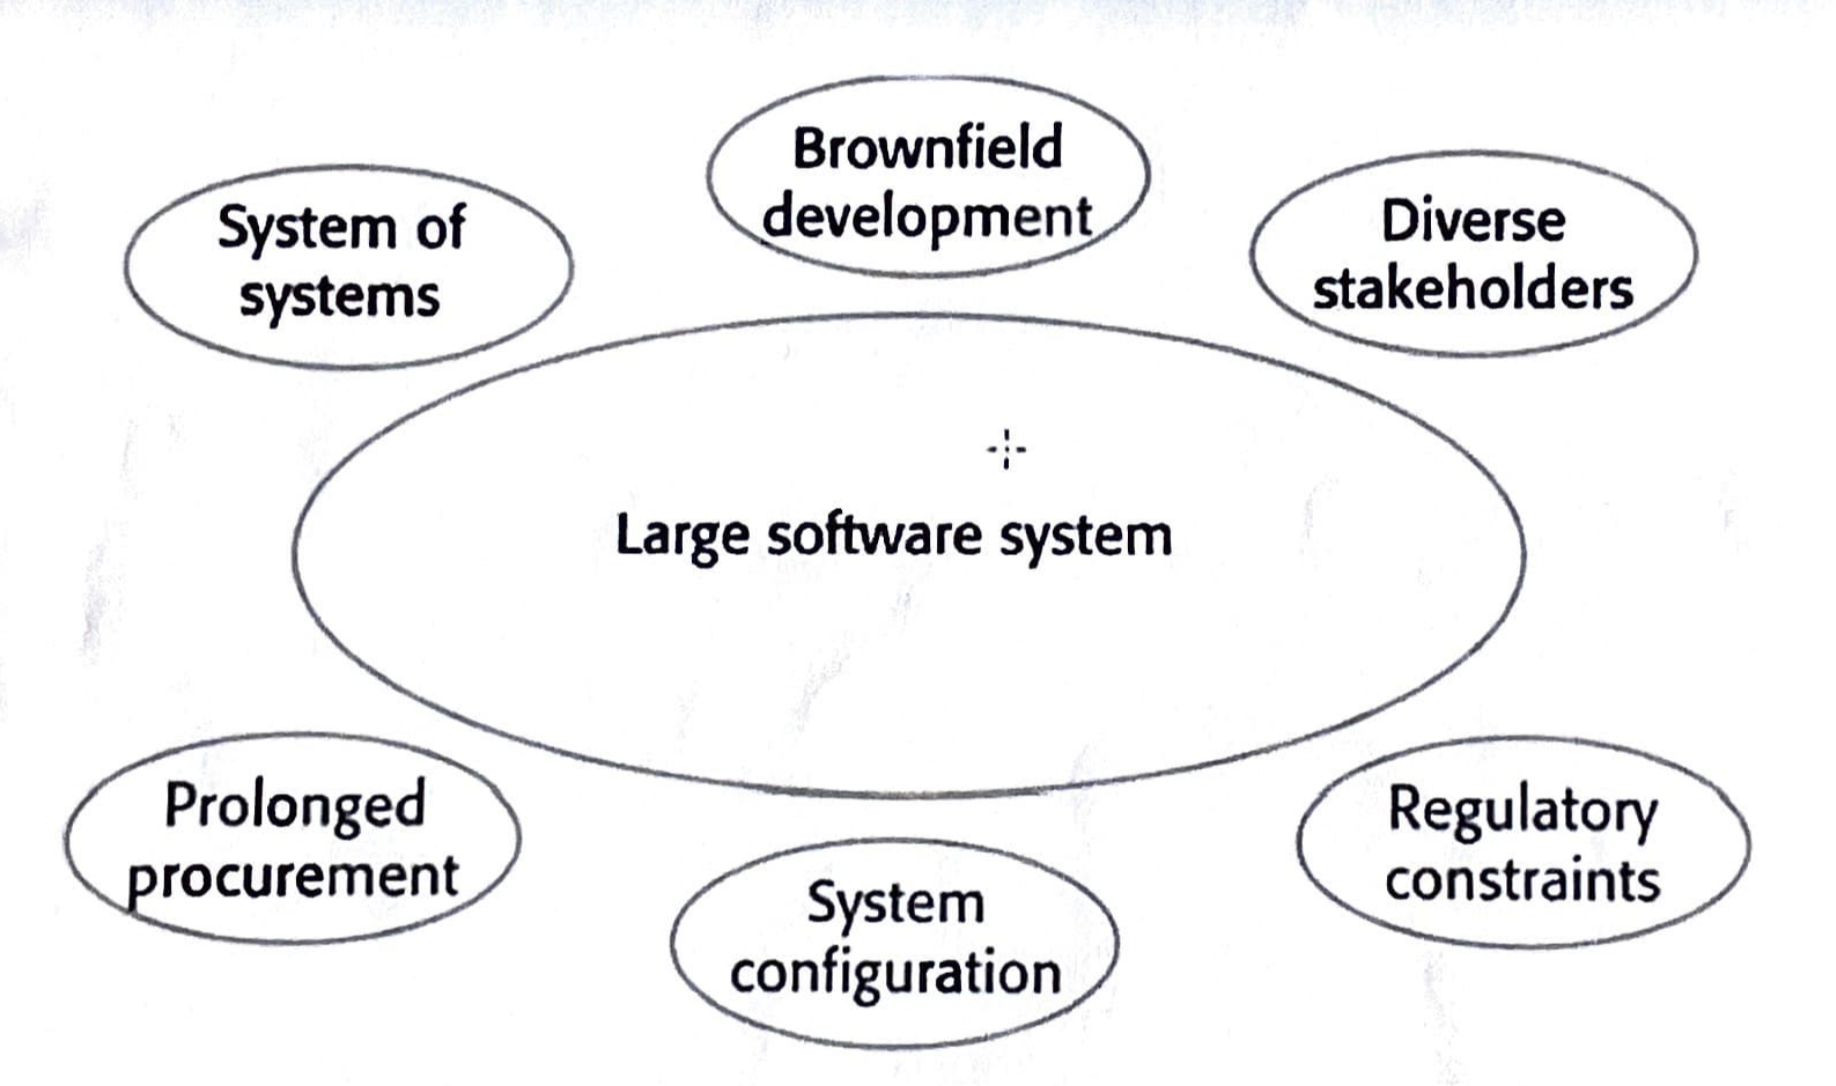
\includegraphics[width=0.75\linewidth]{assets/large-software.png}
    \label{fig:large-software}
\end{figure}

\newpage
Adattare le metodologie agili allo sviluppo di sistemi di grandi dimensioni è molto difficoltoso. La soluzione sta nell'adottare un compromesso tra metodologie tradizioni (pianificate) e metodologie agili, scegliendo quando aderire ad una piuttosto che all'altra sulla base di:
\begin{itemize}
    \item \textbf{Tipologia del software}: dimensioni, grado di progettazione/documentazione richiesto, tempo di vita, eventuali regolamentazioni esterne;
    \item \textbf{Caratteristiche del team} di sviluppo: competenze, distribuzione del personale, tecnologie adottate, ecc...
    \item \textbf{Tradizione dell'organizzazione}: esigenze contrattuali, pratiche di business/marketing, esperienze passate e standard aziendali.
\end{itemize}

\section{Design by Contract}

\paragraph{Design by Contract} Metodologia basata sulla metafora di un \textit{contratto legale}. Avviene un accordo formale tra progettisti e committenti in cui si stabiliscono diritti e obbligazioni delle due parti. Per ogni modulo di definisce un \textbf{\textit{contratto}} (specifica funzionale) che stabilisce richieste e responsabilità. Ne conseguono maggiore \textit{corretteza} e \textit{robustezza}.

\subsection{Concetti alla base del DBC}

\paragraph{Pre-condizioni} Proprietà booleane che devono risultare \textbf{vere PRIMA dell'esecuzione} di un'operazione. Sono \textbf{responsabilità di chi invoca l'operazione}. Si basano su: stato corrente dell'oggetto e parametri in ingresso.

\paragraph{Post-condizioni} Proprietà booleane che devono risultare \textbf{vere DOPO dell'esecuzione} di un'operazione. Sono \textbf{responsabilità di chi implementa l'operazione}. Si basano su: stato dell'oggetto durante invocazione e a valle dell'esecuzione, parametri in ingresso e valore restituito.

\paragraph{Tripla di Hoare} \{$P$\} $op$ \{$Q$\}\\
$P$ è dominio dei valori che soddisfano la pre-condizione\\
$Q$ è dominio dei valori che soddisfano la post-condizione\\
L'implementazione dell'operazione $op$ è corretta se e solo se:
\begin{itemize}
    \item $P$ è corretta prima dell'avvio dell'esecuzione
    \item $Q$ è corretta prima del termine dell'esecuzione
\end{itemize}

\paragraph{Forza delle condizioni} Una pre/post-condizione si dice:
\begin{itemize}
    \item \textbf{stronger} se si restringe il dominio di valori per cui è vera (caso limite: \textit{false})
    \item \textbf{weaker} se si allarga il dominio di valori per cui è vera (caso limite: \textit{true})
\end{itemize}

\begin{center}
Se $P$ $\subseteq$ $Q$ allora $P$ è più forte di $Q$.
\end{center}

Date \textit{$P_1$} e \textit{$P_2$}, $P_1$ è più forte di $P_2$ se $P_1 \Rightarrow P_2$:
\begin{itemize}
    \item Se $P_1$ è vera allora anche $P_2$ è vera
    \item Se $P_1$ è falsa allora $P_2$ non è per forza falsa
    \item $\{false\} \Rightarrow ... \Rightarrow P_1 \Rightarrow P_2 \Rightarrow ... \Rightarrow \{true\}$
\end{itemize}

\paragraph{Linguaggio Eiffel} Implementa il DBC tramite notazione esplicita quale:
\begin{verbatim}
    require P
    A
    require Q
\end{verbatim}
Ogni esecuzione di $A$ richiede che $P$ sia soddisfatta prima dell'esecuzione e che $Q$ sia soddisfatta al termine dell'operazione. Le condizioni si verificano tramite \textbf{asserzioni}, se queste non sono verificate allora si dice che l'operazione viene eseguita \textbf{al di fuori del contratto} (senza garanzie). In tal caso vengono sollevate \textbf{eccezioni}, la loro gestione (\textit{exception handling}) riguarda la robustezza.

\paragraph{Invariante di classe} condizione logica che stabilisce quali sono gli stati ammissibili per gli oggetti istanze di una classe (non durante l'esecuzione di un metodo). Si basa soltanto sullo stato dell'oggetto, ad esempio: \textit{avendo una classe che rappresenta un triangolo, l'invariante sarebbe che i tre punti che lo compongono non siano allineati nel piano cartesiano}.

\newpage

\textbf{Formalmente}:

Data una classe $C$, un'invariante $inv$ è corretta se per ogni costruttore $c$ con argomenti $arg_c$ si ha che:
\begin{center}
    $\{default \land pre(arg_c)\}\ c_{body}\ \{post(arg_c) \land inv\}$
\end{center}
Allo stesso modo, per ogni metodo public $m$ con argomenti $arg_m$, un'invariante $inv$ è corretta se:
\begin{center}
    $\{pre(arg_c) \land inv\}\ m_{body}\ \{post(arg_m) \land inv\}$
\end{center}
\begin{itemize}
    \item I metodi privati non hanno obblighi di verifica dell'invariante
    \item L'invariante è un vincolo sugli stati visibili
    \item Bisogna garantire invisibilità allo stato dell'oggetto durante l'esecuzione
\end{itemize}

\paragraph{Verifica delle condizioni} In Java si fa uso di \textbf{asserzioni}:
\begin{center}
    \begin{lstlisting}[language=Java]
    assert exp: param;    
    \end{lstlisting}
\end{center}
dove \textit{exp} è preposizione booleana e \textit{param} è parametro di \textit{AssertionError} (tipicamente una stringa).

\begin{multicols}{2}
\begin{lstlisting}[language=Java]
m() { 
    ...
    assert inv();
    assert post(); 
}    
\end{lstlisting}
\textit{Approccio standard}
\columnbreak
\begin{lstlisting}[language=Java]
m() {
    if(!pre())
        throw new Exception();
    ...
    assert inv(); 
    assert post(); 
}
\end{lstlisting}
\textit{Approccio difensivo}
\end{multicols}


\subsection{Principio di sostituibilità di Liskov}
\label{liskov}

\paragraph{Definizione} Una classe $D$ derivata da una classe $S$ (superclasse) deve essere progettata in modo tale che gli oggetti di tipo $D$ siano correttamente sostituibili ad oggetti di tipo $S$ in ogni riga di codice dove è attesa un’istanza di classe $S$. Un oggetto di classe $D$ deve essere a tutti gli effetti anche un oggetto di classe $S$, solo un po’ più specializzata

\paragraph{Polimorfismo} Ad un oggetto dichiarato di classe $S$ (tipo statico) può essere assegnata un'istanza di classe $D$ (tipo dinamico)
\begin{center}
\begin{lstlisting}[language=Java]
B b;
D d = new D(); // B extends D
b = d;
\end{lstlisting}
\end{center}
Dunque, se si invoca sull’oggetto $b$ un metodo $m_b$ ridefinito nella classe $D$, la versione di $m_b$ che viene eseguita è quella relativa al tipo dinamico dell’istanza ($m_d$, dynamic binding).

\paragraph{Integrazione del DBC (1)} L’invariante della sottoclasse deve essere compatibile con quello della superclasse. In particolare, per ogni oggetto di classe $D$ deve valere:
\begin{center}
    $inv_b$ AND $inv_D$
\end{center}

\paragraph{Integrazione del DBC (2)} Per ogni metodo $m$ della superclasse ridefinito nella sottoclasse:
\begin{enumerate}
    \item La \textbf{pre-condizione} della sottoclasse deve essere \textbf{più debole} o al più uguale della pre-condizione della superclasse $\{pre_B(m) \Rightarrow pre_D(m)\}$
    \item La \textbf{post-condizione} della sottoclasse deve essere \textbf{più forte} o al più uguale della post-condizione della superclasse $\{post_B(m) \Leftarrow post_D(m)\}$
\end{enumerate}

\paragraph{Esempi} 
\begin{itemize}
    \item Il \textbf{rafforzo} di post-condizione si raggiunge tramite \textit{covarianza} del tipo di ritorno.
    \item L'\textbf{indebolimento} di pre-condizione tramite l'override da \textit{protected} (o \textit{private}) a \textit{public}.
\end{itemize}

\paragraph{Controvarianza} Supportata da alcuni linguaggi. Uso di un oggetto istanza di superclasse $S_T$ al posto dell'oggetto $T$ (indebolimento di pre-condizione)

\newpage